\chapter{Metodología y planificación}
\label{chap:metodologia}

\lettrine{E}{l} desarrollo de un proyecto de software de la envergadura de un Trabajo de Fin de Grado requiere una organización rigurosa para garantizar el cumplimiento de los plazos y la calidad de los entregables. 

\section{Metodología de desarrollo}
Debido a la naturaleza investigadora y de desarrollo individual de este proyecto, no se ha adoptado una metodología ágil estricta (como Scrum), que está más orientada a equipos de desarrollo con roles definidos. 

En su lugar, se ha optado por un enfoque \textit{iterativo e incremental}. Este enfoque permite dividir el ciclo de vida del proyecto en ciclos más cortos y manejables (iteraciones), en cada uno de los cuales se añade funcionalidad o se refinan las características existentes.

Las fases iterativas de este proyecto han sido las siguientes:
\begin{enumerate}
    \item \textbf{Análisis e investigación teórica:} Definición de los factores de riesgo de abandono escolar y estudio de la viabilidad de extracción de datos.
    \item \textbf{Diseño de la arquitectura:} Elección de la pila tecnológica y diseño del ecosistema de contenedores Docker.
    \item \textbf{Modelado de datos:} Diseño del esquema en estrella y mapeo origen-destino.
    \item \textbf{Desarrollo ETL:} Implementación iterativa de los pipelines (extracción de tablas transaccionales, transformación y carga dimensional).
    \item \textbf{Desarrollo backend y frontend:} Exposición de los datos mediante una API RESTful y creación de los \textit{dashboards} visuales, ajustando los umbrales de alerta en base a los resultados observados.
\end{enumerate}

Esta estrategia ha dotado al desarrollo de la flexibilidad necesaria para ajustar las reglas de negocio, como las puntuaciones de riesgo por necesidades educativas especiales o los umbrales socioeconómicos, a medida que se profundizaba en la casuística de los datos reales.

\section{Gestión y control de versiones}
Para el correcto seguimiento de la evolución del proyecto, se ha empleado \textbf{Git} como sistema de control de versiones descentralizado. El repositorio central se ha alojado en GitHub, lo que ha facilitado mantener un histórico organizado de los cambios estructurales.

Siguiendo las mejores prácticas de la industria, el repositorio se estructuró monorepo separando claramente los dominios funcionales en directorios independientes (\textit{api}, \textit{dwh}, \textit{hop}, \textit{frontend}), lo que permitió aplicar la metodología iterativa sobre componentes aislados sin interferir con el resto del ecosistema.

\section{Planificación temporal}

Para el control y la gestión del tiempo del proyecto, se ha diseñado una planificación estructurada en un horizonte temporal de cuatro meses, abarcando desde el inicio de la investigación hasta la defensa final. Esta planificación se ha plasmado visualmente mediante un diagrama de Gantt (ver Figura \ref{fig:gantt}), que permite monitorizar el solapamiento y la dependencia entre las distintas iteraciones de desarrollo.

El cronograma se divide en cinco grandes bloques de trabajo:

\begin{itemize}
    \item \textbf{Fase 1: análisis y diseño (mes 1).} Dedicada a la investigación teórica del problema, la definición de requisitos funcionales y el diseño de la arquitectura tecnológica y el modelo de datos.
    \item \textbf{Fase 2: ingeniería de datos (mes 2).} Centrada en el despliegue del entorno Docker y el desarrollo intensivo de los procesos ETL con Apache Hop.
    \item \textbf{Fase 3: desarrollo backend (mes 3).} Construcción de la API RESTful con FastAPI y las consultas analíticas sobre el Datamart.
    \item \textbf{Fase 4: desarrollo frontend y validación (mes 3--4).} Implementación del cuadro de mando interactivo en React y ejecución de pruebas globales de integración del sistema completo.
    \item \textbf{Fase 5: documentación y cierre (mes 4).} Redacción de la presente memoria académica, revisión de entregables y preparación de la defensa oficial.
\end{itemize}

\begin{figure}[htbp]
    \centering
    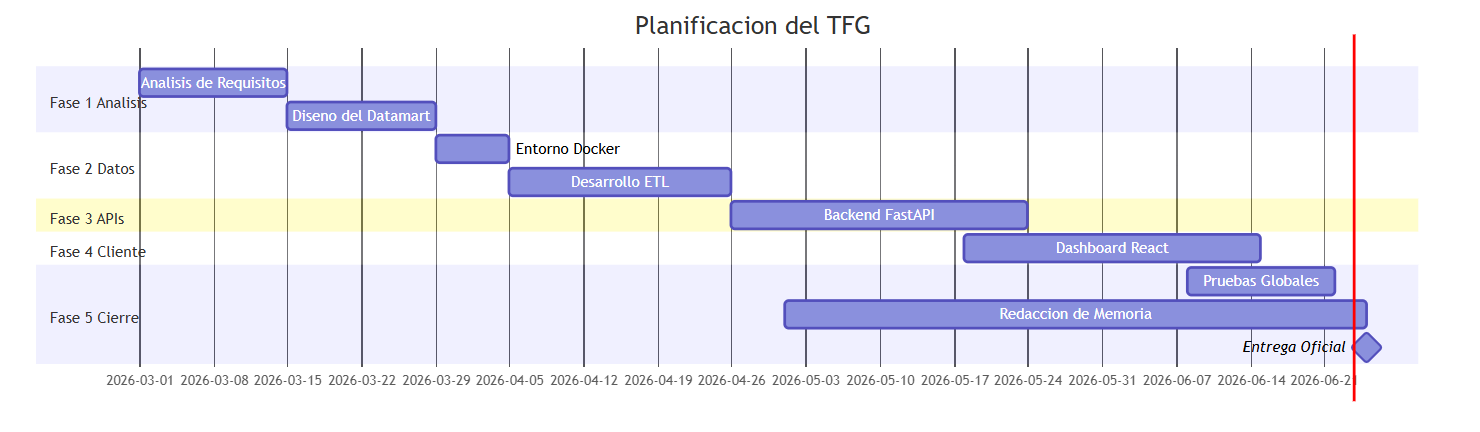
\includegraphics[width=\textwidth]{imaxes/planificacion_gantt.png}
    \caption{Diagrama de Gantt de la planificación del proyecto.}
    \label{fig:gantt}
\end{figure}

\section{Presupuesto y costes}

Todo proyecto de ingeniería de software conlleva un consumo de recursos que debe ser cuantificado para evaluar su viabilidad económica. En este apartado se presenta una estimación del presupuesto del proyecto, dividida en costes de recursos humanos y costes materiales o de infraestructura.

\subsection{Recursos humanos}

El principal coste de este Trabajo de Fin de Grado radica en el tiempo invertido en su investigación, desarrollo y documentación. Para realizar una estimación realista, se ha calculado el coste equivalente en un entorno profesional, asumiendo el rol de un Ingeniero de Software Júnior para el desarrollo, y el rol de un Arquitecto/Director de Proyecto para las labores de tutorización.

Tomando como referencia los salarios medios del sector tecnológico en España, se ha establecido un coste por hora de 20\,€ para el perfil júnior y de 50\,€ para el perfil sénior (tutor). La estimación de horas se ajusta a la carga de trabajo típica de un TFG de esta envergadura (equivalente a 12 créditos ECTS, aproximadamente 300--400 horas de trabajo autónomo).

\begin{table}[htbp]
\begin{center}
    \caption{Estimación de presupuesto de recursos humanos.}
    \label{tab:costes_rrhh}
    \begin{tabular}{lrrr}
        \hline
        \textbf{Rol / Puesto} & \textbf{Coste/hora} & \textbf{Horas trabajadas} & \textbf{Coste total} \\
        \hline
        Programador / Ingeniero Júnior & 20\,€ & 400 & 8.000\,€ \\
        Tutor / Director de Proyecto & 50\,€ & 15 & 750\,€ \\
        \hline
        \textbf{Total estimado} & & & \textbf{8.750\,€} \\
        \hline
    \end{tabular}
\end{center}
\end{table}


\subsection{Recursos materiales e infraestructura}

Una de las decisiones arquitectónicas fundamentales de este proyecto ha sido la adopción exclusiva de tecnologías \textit{Open Source} (PostgreSQL, Apache Hop, FastAPI, React) y el uso de contenedores Docker. Esta estrategia garantiza que la solución pueda ser desplegada y auditada sin incurrir en costes de licenciamiento de software privativo.

Durante la fase de desarrollo, el sistema se ha ejecutado íntegramente en un entorno local, utilizando el equipo informático del autor (cuyo coste de amortización se asume implícito). No obstante, para un despliegue en producción de la herramienta accesible vía web, sería necesario contar con una infraestructura de alojamiento y un dominio seguro. A modo de referencia, se presenta una estimación de los costes de infraestructura mínimos para el primer año de operación en un entorno \textit{Cloud} básico:

\begin{table}[htbp]
\begin{center}
    \caption{Estimación de costes materiales y de infraestructura (1 año).}
    \label{tab:costes_materiales}
    \begin{tabular}{lp{6cm}r}
        \hline
        \textbf{Concepto} & \textbf{Descripción} & \textbf{Coste estimado} \\
        \hline
        Licencias de Software & PostgreSQL, Apache Hop, React, FastAPI & 0,00\,€ \\
        Dominio web (.es) & Registro anual para acceso público y certificados SSL & 12,00\,€ \\
        Servidor Virtual (VPS) & Instancia básica en la nube (ej. 4\,GB RAM, 2 vCPU) a $\sim$15\,€/mes & 180,00\,€ \\
        \hline
        \textbf{Total estimado (1 año)} & & \textbf{192,00\,€} \\
        \hline
    \end{tabular}
\end{center}
\end{table}

En conclusión, el proyecto demuestra una alta viabilidad económica. Al carecer de costes de licencias, la administración pública u organización educativa que desee adoptar esta solución únicamente tendría que asumir los costes de alojamiento en sus propios servidores (o en una nube pública) y el mantenimiento evolutivo del código.
